% !TEX TS-program = lualatex
\documentclass[12pt,a4paper]{article}

% =========================
% Langue + typographie FR
% =========================
\usepackage[french]{babel}
\usepackage{csquotes}
\usepackage{unicode-math}
\setmathfont{GoldmanSans_Rg.ttf}

\usepackage{fontspec}
\defaultfontfeatures{Ligatures=TeX}
\setmainfont{GoldmanSans_Rg.ttf}

\usepackage{microtype}


% =========================
% Mise en page (marges réduites)
% =========================
\usepackage[a4paper,margin=2.3cm]{geometry} % <- plus de surface utile
\setlength{\parindent}{0pt}
\setlength{\parskip}{0.8em}

% =========================
% Packages
% =========================
\usepackage{graphicx}
\usepackage{xcolor}
\usepackage[hidelinks]{hyperref}
\usepackage{tcolorbox}
\tcbuselibrary{skins,breakable}
\usepackage{tikz}
\usepackage{array}
\usepackage{tabularx}
\usepackage{booktabs}

% =========================
% Couleurs
% =========================
\definecolor{canadared}{HTML}{D80621}
\definecolor{ink}{HTML}{111111}
\definecolor{softgray}{HTML}{F4F4F4}

% =========================
% Grandes tailles (comme ton exemple)
% =========================
\newcommand{\YUGE}{\fontsize{44}{52}\selectfont}
\newcommand{\HUGEPLUS}{\fontsize{22}{28}\selectfont}
\newcommand{\BIG}{\fontsize{14}{18}\selectfont}

% =========================
% tcolorbox style
% =========================
\tcbset{
  sharp corners,
  boxrule=0.5pt,
  colframe=black!30,
  colback=gray!5,
  left=2mm,
  right=2mm,
  top=1.5mm,
  bottom=1.5mm,
  breakable
}

% =========================
% Meta
% =========================
\newcommand{\DocTitleA}{TCF}
\newcommand{\DocTitleB}{Canada}
\newcommand{\DocTitleC}{Cheatsheet}

\begin{document}

% =========================
% Titlepage (strictement sur ton modèle)
% =========================
\begin{titlepage}
\begin{tikzpicture}[remember picture, overlay]
    \node[anchor=north west, inner sep=0pt] at (current page.north west) {
        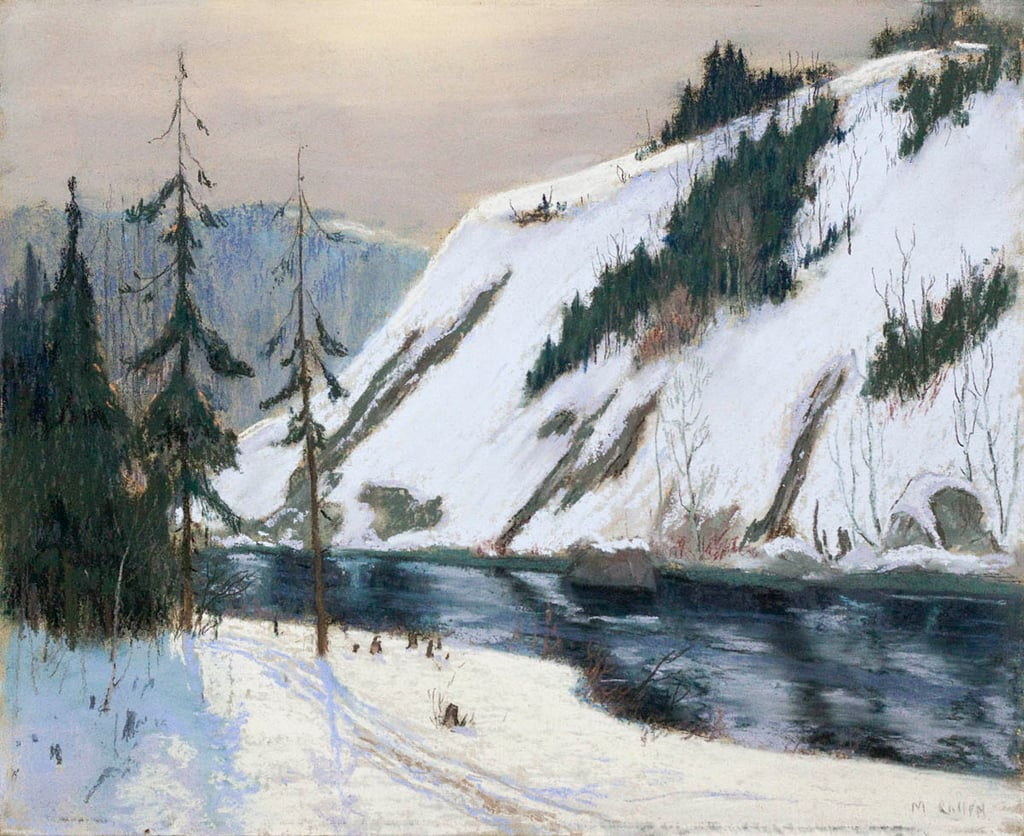
\includegraphics[width=\paperwidth, keepaspectratio=true]{Sunlight on the Snow.jpg}
    };
% Maurice Cullen Sunlight on the Snow- St. Anne's River pastel, circa 1925 15.5 x 18 in (39.4 x 45.7 cm) https://mayberryfineart.com/art/2214851/sunlight-on-the-snow-st-annes-river-maurice-cullen?srsltid=AfmBOopgMpmGsZwadIPzeSvYhkUkHOh3fvTS44Q0EOJznA2Bz2r8Ihbw
    \node[anchor=south west, inner sep=1em, yshift=13em] at (current page.south west) {
        \parbox{\textwidth}{
            \raggedright
            \YUGE \textbf{\textcolor{ink}{\DocTitleA} \textcolor{canadared}{\DocTitleB} \textcolor{ink}{\DocTitleC}}\\
            \vspace{0.8em}
        }
    };
\end{tikzpicture}
\end{titlepage}

% =========================
% Tables de repère (au début)
% =========================
\section*{Repères TCF Canada}
\addcontentsline{toc}{section}{Repères TCF Canada}

\begin{tcolorbox}[title=\textbf{Scores requis (objectif B2) : synthèse}]
\renewcommand{\arraystretch}{1.25}
\begin{tabularx}{\textwidth}{@{}>{\raggedright\arraybackslash}X >{\raggedright\arraybackslash}m{3.8cm} >{\raggedright\arraybackslash}m{2.6cm}@{}}
\toprule
\textbf{Section} & \textbf{Score TCF requis} & \textbf{Échelle} \\
\midrule
Compréhension de l'oral & 458 à 502 & 0 à 699 \\
Compréhension de l'écrit & 453 à 498 & 0 à 699 \\
Expression écrite & 10 à 11 & 0 à 20 \\
Expression orale & 10 à 11 & 0 à 20 \\
\bottomrule
\end{tabularx}
\end{tcolorbox}

\begin{tcolorbox}[title=\textbf{Format des épreuves (durée, tâches, barèmes)}]
\renewcommand{\arraystretch}{1.25}
\begin{tabularx}{\textwidth}{@{}>{\raggedright\arraybackslash}m{1.2cm} >{\raggedright\arraybackslash}m{3.3cm} >{\raggedright\arraybackslash}X@{}}
\toprule
\textbf{Code} & \textbf{Durée / volume} & \textbf{Détails}\\
\midrule
CO & 35 min / 39 q. & Compréhension de l'oral\\
\midrule
CÉ & 60 min / 39 q. & \textbf{Compréhension écrite : correspondances indicatives}\\
\multicolumn{3}{@{}l@{}}{\vspace{-0.2em}}\\
\multicolumn{3}{@{}l@{}}{%
\renewcommand{\arraystretch}{1.2}
\begin{tabularx}{\textwidth}{@{}m{4.2cm} m{2.2cm} m{3.0cm} X@{}}
\toprule
\textbf{Plage de questions} & \textbf{Score} & \textbf{Total de points} & \textbf{Repère} \\
\midrule
1--4   & 3  & 4 × 3 = 12    & TCF Canada Compréhension écrite \\
5--10  & 9  & 6 × 9 = 54    &  \\
11--19 & 15 & 9 × 15 = 135  &  \\
20--29 & 21 & 10 × 21 = 210 &  \\
30--35 & 26 & 6 × 26 = 156  &  \\
36--39 & 33 & 4 × 33 = 132  &  \\
\bottomrule
\end{tabularx}
}\\
\midrule
EÉ & 60 min / 3 t. & \textbf{Expression écrite}\\
\multicolumn{3}{@{}l@{}}{\vspace{-0.2em}}\\
\multicolumn{3}{@{}l@{}}{%
\renewcommand{\arraystretch}{1.2}
\begin{tabularx}{\textwidth}{@{}m{2.2cm} m{3.0cm} X@{}}
\toprule
\textbf{Tâche} & \textbf{Longueur} & \textbf{Repère}\\
\midrule
Tâche 1 & 60--120 m.   & TCF Canada Expression écrite\\
Tâche 2 & 120--150 m.  & \\
Tâche 3 & 120--180 m.  & \\
\bottomrule
\end{tabularx}
}\\
\midrule
EO & 12 min / 3 t. & \textbf{Expression orale}\\
\multicolumn{3}{@{}l@{}}{\vspace{-0.2em}}\\
\multicolumn{3}{@{}l@{}}{%
\renewcommand{\arraystretch}{1.2}
\begin{tabularx}{\textwidth}{@{}m{2.2cm} m{3.0cm} X@{}}
\toprule
\textbf{Tâche} & \textbf{Durée} & \textbf{Repère}\\
\midrule
Tâche 1 & 2 min      & TCF Canada Expression orale\\
Tâche 2 & Préparation 2 min + Durée de l'échange 3 min 30   & \\
Tâche 3 & 4 min 30   & \\
\bottomrule
\end{tabularx}
}
\\
\bottomrule
\end{tabularx}
\end{tcolorbox}

\clearpage

% =========================
% Table des matières
% =========================
\tableofcontents
\clearpage

% =========================
% Expression écrite (EÉ)
% =========================
\section{Expression écrite (EÉ)}

\subsection{Tâche 1 — Message descriptif : décrire, raconter, expliquer}

% =========================================================
% VERSION INFORMELLE (amis, proches) — C1 stabilisé
% =========================================================

\begin{tcolorbox}[title=\textbf{VERSION INFORMELLE · C1 (amis / proches)}]

\textbf{STEP 1 · Mise en situation (1 à 2 phrases)}
\emph{Objectif : identifier clairement le destinataire et l'intention, avec un rappel de contexte si utile.}
\begin{itemize}
  \item Salut + prénom,
  \item \textbf{Je t'écris pour} + annoncer l'objectif (inviter / informer / expliquer / demander).
  \item (Option) \textbf{Comme tu me l'as demandé / Puisque tu voulais savoir…}
\end{itemize}

\textbf{STEP 2 · Contenu principal structuré (3 à 5 phrases)}
\emph{Objectif : donner des informations concrètes et organisées.}
\begin{itemize}
  \item \textbf{Il s'agit de…} + description précise (lieu, date, horaire, prix, etc.).
  \item \textbf{Ce qui est intéressant, c'est que…} + avantage clé / détail utile.
  \item \textbf{Non seulement…, mais en plus…} + 2e avantage (option).
  \item \textbf{On y trouve / On y fait…} + activités / services / éléments pratiques.
  \item \textbf{Au programme : …} + liste courte et claire (option).
\end{itemize}

\textbf{STEP 3 · Avis + justification + comparaison (2 à 3 phrases)}
\emph{Objectif : évaluer, justifier, comparer (marqueur C1).}
\begin{itemize}
  \item \textbf{Je pense que… / Je trouve que…} + justification (\textbf{car / puisque…}).
  \item \textbf{Bien que…}, + idée principale (nuance / concession).
  \item \textbf{Comparé(e) à…}, + avantage / différence.
  \item \textbf{À mon avis, cela permet de…} + bénéfice concret.
\end{itemize}

\textbf{STEP 4 · Clôture interactionnelle (1 à 2 phrases)}
\emph{Objectif : conclure comme un échange réel et obtenir une réponse.}
\begin{itemize}
  \item \textbf{Dis-moi si cela te convient / si tu es partant.}
  \item \textbf{N'hésite pas à me dire si tu as une question.}
  \item \textbf{À bientôt / À très bientôt.}
\end{itemize}

\end{tcolorbox}


% =========================================================
% VERSION FORMELLE (journal, agence, entreprise) — C1 structuré
% =========================================================

\begin{tcolorbox}[title=\textbf{VERSION FORMELLE · C1 (professionnel / institution)}]

\textbf{STEP 1 · Introduction professionnelle (1 à 2 phrases)}
\emph{Objectif : présenter la demande de manière polie et contextualisée.}
\begin{itemize}
  \item Madame, Monsieur,
  \item \textbf{Je me permets de vous contacter afin de…} (informer / demander / proposer).
  \item (Option) \textbf{Dans le cadre de…} + contexte.
\end{itemize}

\textbf{STEP 2 · Développement structuré (3 à 5 phrases)}
\emph{Objectif : fournir les informations utiles avec des connecteurs.}
\begin{itemize}
  \item \textbf{Il s'agit de…} + description précise et contextualisée.
  \item \textbf{Ce projet / ce bien / ce poste présente plusieurs avantages, notamment…}
  \item \textbf{En effet…} + précision factuelle.
  \item \textbf{Par ailleurs…} + information complémentaire (prix, disponibilité, conditions, etc.).
\end{itemize}

\textbf{STEP 3 · Positionnement (2 à 3 phrases)}
\emph{Objectif : exprimer un avis argumenté et nuancé.}
\begin{itemize}
  \item \textbf{À mon sens… / Il me semble pertinent de…}
  \item \textbf{Bien que…}, \textbf{il convient de…} + nuance / recommandation.
  \item \textbf{Comparé(e) à…}, + justification (option).
\end{itemize}

\textbf{STEP 4 · Clôture professionnelle (1 à 2 phrases)}
\emph{Objectif : conclure clairement et ouvrir vers la suite.}
\begin{itemize}
  \item \textbf{Je reste à votre disposition pour toute information complémentaire.}
  \item \textbf{Dans l'attente de votre retour,} \textbf{bien cordialement.}
  \item (Option très formelle) \textbf{Je vous prie d'agréer, Madame, Monsieur, l'expression de mes salutations distinguées.}
\end{itemize}

\end{tcolorbox}


\subsection{Tâche 2 — Raconter une expérience et exprimer une attitude personnelle}

\begin{tcolorbox}[title=\textbf{REPÈRE GLOBAL — Ce que l'examinateur attend réellement}]
\emph{
La Tâche 2 évalue votre capacité à :
\begin{itemize}
  \item raconter une expérience vécue de manière claire et structurée ;
  \item décrire des faits concrets (et non abstraits) ;
  \item exprimer un ressenti personnel nuancé ;
  \item introduire éventuellement une limite sans développer une argumentation formelle.
\end{itemize}
L'objectif n'est pas de débattre, mais de montrer une narration organisée et une réflexion personnelle maîtrisée.
}
\end{tcolorbox}

% ----------------------------------------------------

\begin{tcolorbox}[title=\textbf{STEP 1 · Situer clairement le contexte (1–2 phrases)}]
\emph{Objectif : préciser le moment, le lieu et l'intention.}

\begin{itemize}
  \item Le week-end dernier / Il y a quelques semaines…
  \item J'ai eu l'occasion de…
  \item Cette initiative avait pour objectif de…
  \item J'étais curieux(se) de…
  \item Je souhaitais…
\end{itemize}

\textbf{Conseil :} Mentionner le cadre + une motivation rend l'introduction plus naturelle et plus crédible.
\end{tcolorbox}

% ----------------------------------------------------

\begin{tcolorbox}[title=\textbf{STEP 2 · Décrire le déroulement concret (3–4 phrases)}]
\emph{Objectif : raconter avec des actions précises et des éléments concrets.}

\begin{itemize}
  \item D'abord… Ensuite… Enfin…
  \item Au cours de la journée…
  \item Les activités consistaient à…
  \item J'ai notamment participé à…
  \item Cette situation m'a confronté(e) à…
\end{itemize}

\textbf{Attention :} éviter les phrases vagues comme ``c'était intéressant''.  
Toujours préciser : quoi ? comment ? avec qui ? dans quel contexte ?
\end{tcolorbox}

% ----------------------------------------------------

\begin{tcolorbox}[title=\textbf{STEP 3 · Exprimer le ressenti personnel (2–3 phrases)}]
\emph{Objectif : montrer votre position personnelle et votre évolution.}

\begin{itemize}
  \item Personnellement, j'ai particulièrement apprécié…
  \item Ce que j'ai trouvé le plus intéressant, c'est…
  \item Cette expérience m'a permis de…
  \item Elle m'a fait prendre conscience de…
  \item Elle m'a aidé(e) à développer…
\end{itemize}

\textbf{Conseil C1 :} privilégier les verbes d'évolution (m'a amené à, m'a obligé à, m'a appris à).
\end{tcolorbox}

% ----------------------------------------------------

\begin{tcolorbox}[title=\textbf{STEP 4 · Introduire une limite maîtrisée (facultatif mais valorisant)}]
\emph{Objectif : apporter de la nuance sans créer un débat.}

\begin{itemize}
  \item Bien sûr, tout n'était pas parfait.
  \item Certains aspects étaient plus difficiles…
  \item Il faut reconnaître que…
  \item L'organisation laissait à désirer.
\end{itemize}

\textbf{Principe :} Mentionner brièvement une limite puis revenir à l'évaluation globale.
\end{tcolorbox}

% ----------------------------------------------------

\begin{tcolorbox}[title=\textbf{STEP 5 · Conclure avec une appréciation globale (1 phrase)}]
\emph{Objectif : synthétiser l'expérience sans introduire de nouvelle idée.}

\begin{itemize}
  \item Dans l'ensemble…
  \item Avec le recul…
  \item Malgré cela…
  \item Je garde un souvenir…
  \item Je considère que…
\end{itemize}

\textbf{Règle :} conclusion brève, claire et cohérente avec le ressenti exprimé.
\end{tcolorbox}

% ----------------------------------------------------

\begin{tcolorbox}[title=\textbf{RÉPARTITION IDÉALE (120–150 mots)}]
\begin{itemize}
  \item Introduction (contexte) : 20–30 mots
  \item Déroulement concret : 50–60 mots
  \item Ressenti personnel : 30–40 mots
  \item Limite : 15–20 mots
  \item Conclusion : 10–15 mots
\end{itemize}

\textbf{Total conseillé : 135–145 mots.}
\end{tcolorbox}

\subsection{Tâche 3 — Synthèse comparative + prise de position}

% =========================================================
% INTRODUCTION : Mise en perspective des deux documents
% =========================================================

\begin{tcolorbox}[title=\textbf{STEP 1 · Introduction comparative}]

\begin{itemize}
  \item La question de \dots\ suscite aujourd'hui des positions contrastées.
  \item Le document 1 met en avant \dots, en insistant notamment sur \dots.
  \item À l'inverse, le document 2 souligne \dots, en mettant l'accent sur \dots.
  \item Ainsi, les deux textes proposent des visions différentes de \dots.
\end{itemize}

\emph{Objectif : reformuler les deux documents de manière équilibrée, sans juger.}

\end{tcolorbox}


% =========================================================
% DÉVELOPPEMENT : Analyse + prise de position nuancée
% =========================================================

\begin{tcolorbox}[title=\textbf{STEP 2 · Analyse et position argumentée}]

\begin{itemize}
  \item Sans opposer ces deux perspectives de manière rigide, il apparaît que \dots.
  \item Je me rapproche davantage de l'analyse du document X, dans la mesure où \dots.
  \item Lorsqu'elle est encadrée / mise en œuvre de façon réfléchie, cette pratique peut \dots.
  \item Toutefois, les réserves exprimées dans le document Y demeurent pertinentes, notamment en ce qui concerne \dots.
  \item Une approche équilibrée permettrait ainsi de concilier \dots\ et \dots.
\end{itemize}

\emph{Objectif :}
\begin{itemize}
  \item Prendre position clairement
  \item Reconnaître les limites
  \item Introduire une condition ou un cadre
  \item Montrer une capacité de synthèse
\end{itemize}

\end{tcolorbox}


% =========================================================
% CONCLUSION : Ouverture + généralisation
% =========================================================

\begin{tcolorbox}[title=\textbf{STEP 3 · Conclusion structurée}]

\begin{itemize}
  \item En définitive, bien que les deux points de vue soient recevables, \dots.
  \item La pertinence de cette pratique dépend avant tout des conditions de sa mise en œuvre.
  \item À long terme, une régulation adaptée permettrait de \dots.
  \item Cette réflexion invite à repenser \dots\ dans une perspective plus durable et équilibrée.
\end{itemize}

\emph{Objectif : généraliser sans répéter les arguments.}

\end{tcolorbox}

% =========================
% Expression orale (EO)
% =========================
\section{Expression orale (EO)}

\subsection{Tâche 1 — Présentation personnelle}

\begin{tcolorbox}[title=\textbf{Présentation formelle ($\approx$ 1 min)}]
Bonjour Madame, bonjour Monsieur, // \\

Je m'appelle Léo, j'ai vingt-six ans // et je viens de la province du Jiangsu, en Chine. // \\

J'ai fait mes études en informatique à l'Université normale de la Chine de l'Est, // où j'ai obtenu une licence puis un master. // \\
Aujourd'hui, je travaille comme ingénieur en développement mobile // dans une grande entreprise technologique. // \\

Dans mon travail, // ce qui m'intéresse particulièrement, // c'est le fait de résoudre des problèmes concrets // et d'améliorer l'expérience des utilisateurs // grâce à la technologie. // \\

À côté de ça, // j'apprends le français depuis environ un an. // \\
Au début, mon objectif était assez \textbf{pragmatique} : // \\
je souhaite m'installer au \textbf{Canada} à long terme, // \\
et le français est \textbf{indispensable} pour m'intégrer, // notamment au \textbf{Québec}. // \\

Mais avec le temps, // cet apprentissage est devenu bien plus qu'un simple objectif pratique : // \\
j'ai développé un réel intérêt // pour la culture et l'histoire francophones, // notamment la \textbf{Révolution française}. // \\

Ce qui me fascine, // c'est la manière dont cette période a transformé la société, // \\
en mettant en avant des valeurs comme la \textbf{liberté}, // l'\textbf{égalité} // et la souveraineté du peuple. // \\
Je m'intéresse aussi aux idées des philosophes des Lumières, // que je trouve encore très pertinentes aujourd'hui. // \\

À l'avenir, // j'aimerais visiter la France et le Canada // pour découvrir des lieux historiques // et mieux comprendre la culture sur place. // \\

En dehors du travail, // je m'intéresse également à l'actualité économique // et aux marchés financiers, // \\
un domaine que je trouve à la fois complexe // et passionnant. // \\

Je dirais que je suis quelqu'un de curieux, // discipliné, // et toujours prêt à apprendre de nouvelles choses. // \\

Je vous remercie pour votre attention. //
\end{tcolorbox}

\subsection{Tâche 2 — Interaction guidée}

\begin{tcolorbox}[title=\textbf{STEP 1 · Entrée en interaction ($\approx$ 20–30 secondes)}]
\emph{Objectif : installer le cadre, rappeler la situation, annoncer la demande.}
\textbf{Formules C1 naturelles}
\begin{itemize}
  \item Bonjour, j'aurais besoin de quelques renseignements.
  \item Comme je vous l'ai expliqué, je souhaiterais…
  \item Je voulais justement vous poser quelques questions à ce sujet.
\end{itemize}
\end{tcolorbox}

\begin{tcolorbox}[title=\textbf{STEP 2 · Questions générales ($\approx$ 1 minute)}]
\emph{Objectif : obtenir une vue d'ensemble avant d'entrer dans les détails.}
\textbf{Questions types}
\begin{itemize}
  \item De quoi s'agit-il exactement ?
  \item Comment cela se passe en général ?
  \item À qui s'adresse cette activité / ce service ?
\end{itemize}
\end{tcolorbox}

\begin{tcolorbox}[title=\textbf{STEP 3 · Questions ciblées et progressives ($\approx$ 1 min 30)}]
\emph{Objectif : approfondir avec des questions précises, organisées par thème.}

\textbf{Organisation générale}
\begin{itemize}
  \item Comment cela s'organise-t-il concrètement ?
  \item Combien de temps cela dure-t-il en général ?
\end{itemize}

\textbf{Horaires / fréquence}
\begin{itemize}
  \item À quelle fréquence ?
  \item Y a-t-il des horaires fixes ?
\end{itemize}

\textbf{Prix / conditions}
\begin{itemize}
  \item Quels sont les tarifs ?
  \item Est-ce qu'il y a des frais supplémentaires ?
\end{itemize}

\textbf{Expérience personnelle}
\begin{itemize}
  \item Et de votre côté, qu'en avez-vous pensé ?
  \item Est-ce que vous recommanderiez cette option ?
\end{itemize}
\end{tcolorbox}

\begin{tcolorbox}[title=\textbf{STEP 4 · Réactions et relances (tout au long de l'échange)}]
\emph{Objectif : montrer la compréhension et construire l'échange.}
\textbf{Formules indispensables}
\begin{itemize}
  \item D'accord, je vois.
  \item C'est intéressant.
  \item Si je comprends bien…
  \item Cela correspond exactement à ce que je cherche.
\end{itemize}
\end{tcolorbox}

\begin{tcolorbox}[title=\textbf{STEP 5 · Clôture claire ($\approx$ 20–30 secondes)}]
\emph{Objectif : conclure naturellement.}
\textbf{Formules efficaces}
\begin{itemize}
  \item Merci pour toutes ces informations.
  \item Cela m'aide beaucoup à y voir plus clair.
  \item Je vais y réfléchir et je vous recontacte si besoin.
\end{itemize}
\end{tcolorbox}

\subsection{Tâche 3 — Expression d'opinion argumentée}

\begin{tcolorbox}[title=\textbf{ÉTAPE 1 · Cadrage du débat + position ($\approx$ 45 s)}]
Alors, globalement, je dirais que c'est une question assez complexe, qui ne se prête pas à une réponse toute faite.

Si on prend un peu de recul, on se rend compte que les avis sont très partagés, notamment parce que les situations varient selon les contextes sociaux, économiques ou culturels.

Quand on y réfléchit, ce débat touche à des enjeux à la fois individuels et collectifs.

À titre personnel, j'ai plutôt tendance à penser que…, même si cette position mérite d'être nuancée.
\end{tcolorbox}

\begin{tcolorbox}[title=\textbf{ÉTAPE 2 · Axe principal : analyse en profondeur ($\approx$ 1 min 30)}]
Déjà, il faut partir d'un constat assez simple : …

Dans les faits, on observe que …, ce qui montre que …

Concrètement, ce que cela implique, c'est que …, tant au niveau des comportements individuels que des dynamiques collectives.

On se rend compte que ce phénomène s'inscrit dans un cadre plus large.

Derrière cela, il y a surtout une logique de …, qu'elle soit sociale, économique ou humaine.
\end{tcolorbox}

\begin{tcolorbox}[title=\textbf{ÉTAPE 3 · Second angle, exemple et nuance ($\approx$ 1 min 30)}]
\textbf{Transition naturelle}
\begin{itemize}
  \item Après, il y a aussi un autre aspect qu'on a tendance à sous-estimer.
  \item Au-delà de cette première lecture, il ne faut pas négliger le fait que …
\end{itemize}

\textbf{Exemple concret}
\begin{itemize}
  \item On le voit très clairement, par exemple, quand …
  \item Typiquement, dans certaines situations, …
\end{itemize}

\textbf{Nuance}
\begin{itemize}
  \item Il ne faut pas non plus idéaliser cette réalité.
  \item Il existe des limites à cette approche, en particulier lorsque …
\end{itemize}

\textbf{Recentrage}
\begin{itemize}
  \item Cela étant dit, l'idée de fond reste la même.
  \item Même en tenant compte de ces limites, je reste convaincu que …
\end{itemize}
\end{tcolorbox}

\begin{tcolorbox}[title=\textbf{ÉTAPE 4 · Conclusion contrôlée ($\approx$ 50 s)}]
Donc, au final, je dirais que cette question ne peut pas être tranchée de manière binaire.

L'enjeu principal consiste à comprendre dans quelles conditions cela peut fonctionner.

En définitive, ce qui compte, c'est de trouver un équilibre réaliste, durable et cohérent avec les besoins de la société actuelle.
\end{tcolorbox}

\begin{tcolorbox}[title=\textbf{Remplissages d'urgence (fluidité orale)}]
\begin{itemize}
  \item Comment dire…
  \item Ce que je veux dire, c'est que…
  \item Si je reformule…
  \item Il faut replacer ça dans un contexte plus large…
  \item Autrement dit…
\end{itemize}
\end{tcolorbox}

\end{document}
